\documentclass[agriengineering,article,submit,moreauthors]{Definitions/mdpi}
\graphicspath{{../papers/figures/}}
\setlength{\headheight}{20pt}
\firstpage{1}
\makeatletter
\setcounter{page}{\@firstpage}
\makeatother
\pubvolume{1}
\issuenum{1}
\articlenumber{0}
\pubyear{2026}
\copyrightyear{2026}
\Title{Strictly Causal Energy-Management Benchmarking for a Hybrid Agricultural Tractor: Map Sensitivity and Controller Feasibility}
\newcommand{\orcidauthorA}{0009-0005-1928-6218}
\Author{Chenyu Cui$^{1}$, Zhenhua Zhu$^{1}$, Lihan Wang$^{1}$, Zaiwang Lu$^{1}$ and Yucheng Zhang$^{1,}$*\orcidA{}}
\AuthorNames{Chenyu Cui, Zhenhua Zhu, Lihan Wang, Zaiwang Lu and Yucheng Zhang}
\address{%
$^{1}$ \quad Prospective Research Laboratory, Institute of Computing Technology, Chinese Academy of Sciences, Beijing 100190, China}
\corres{Correspondence: zhangyucheng@ict.ac.cn}
\datereceived{}
\daterevised{}
\dateaccepted{}
\datepublished{}
\abstract{Reported fuel savings for hybrid agricultural tractors can be dominated by terminal-energy accounting, component-map assumptions, and whether an online controller is truly feasible. This theoretical simulation compares a map-aware equivalent-consumption minimization strategy (ECMS), a public-phase causal policy, deterministic model predictive control (MPC), scenario MPC, and terminal-set safeguarded scenario MPC in a reproducible parameterized OS-ECVT virtual prototype. Every online method shares a defined 300 kW virtual powertrain, a 60 kW stable engine-power floor, a 40 kW s$^{-1}$ applied-output ramp, 150 kW motor and battery-bus limits, proxy MG limits, and a terminal state-of-charge (SOC) error no larger than $10^{-4}$. Ten predeclared ECMS factors are selected on six development seeds and frozen before a 20-seed, 600 s stochastic-cycle test; no controller observes future samples from an evaluated seed. The terminal-set MPC projects its action into the measured-load ramp/electrical set and requires its successor SOC to remain in a terminal-energy viability envelope. Under a literature-shaped efficiency map, ECMS increased paired fuel use by 0.251\% (95\% CI: 0.238\%--0.264\%), the phase policy saved 0.010\% (0.006\%--0.015\%), and terminal-set MPC increased fuel use by 0.704\% (0.653\%--0.756\%) while achieving 20/20 zero-external-fallback, zero-terminal-set-violation paths. Under a deliberately specified steep low-load efficiency-island sensitivity, frozen ECMS saved 10.491\% (10.445\%--10.538\%) on all 20 pairs, whereas all MPC variants remained fuel-inferior. A predeclared horizon--preview mechanism map selected the same eight-sample history-only terminal-set MPC on new development seeds; its 20-seed holdout fuel changes were $-0.168\%$ and $-2.079\%$, respectively. Thus, the terminal-set structure makes the safety policy auditable rather than delegating an empty candidate set to the experiment runner, but does not itself yield fuel savings; virtual controller rankings remain conditional on the declared component maps.}
\keyword{hybrid electric tractor; energy management; ECMS; model predictive control; state of charge; map sensitivity; virtual prototype}
\begin{document}

\section{Introduction}
Agricultural traction demand varies with soil, grade, vehicle speed, implement operation, and auxiliary loads. A hybrid powertrain can buffer this variation, but it can also produce misleading savings when battery depletion, power shortage, or an unfavorable baseline is not controlled. Dynamic programming (DP) is useful as an offline reference \cite{xie2016}, whereas MPC can react to predicted load changes. Existing hybrid-tractor studies have reported substantial but non-comparable savings because their architectures, drive cycles, initial/final SOC conditions, and baselines differ \cite{curiel2023,mocera2020,mocera2020b}.

This article asks two engineering questions. First, when the information set, terminal energy, actuator limits, and baseline are fixed, which causal controller remains both feasible and fuel-competitive? Second, does this answer persist when a literature-shaped engine-efficiency map is contrasted with a deliberately steep low-load sensitivity map on the same virtual hardware? The second question is essential: engine load and rated-power matching affect tractor fuel use \cite{jilek2008,janulevicius2010}, while steady maps omit turbocharger and other transient limits \cite{huo2018}. Accordingly, a virtual fuel-saving result must be interpreted as conditional on its map rather than as a vehicle-performance estimate.

The contributions are as follows: (i) a reproducible OS-ECVT virtual prototype with a strict terminal-energy and hard-constraint rule; (ii) a common causal comparison of map-aware ECMS, a public-phase policy, deterministic MPC, scenario MPC, and terminal-set safeguarded scenario MPC; (iii) development/test separation for the only tuned ECMS parameter; (iv) an auditable conditional recursive-feasibility construction that separates internal safety-filter interventions from experiment-runner fallback; (v) an explicitly labeled map-mechanism sensitivity on the same 300 kW virtual hardware; and (vi) a predeclared horizon--preview mechanism map with an additional development/holdout split. Offline dynamic programming is not included in the online statistics because it has access to future demand. The scope is deliberately limited to simulation. The component maps are defined virtual-model inputs, not claims of field, vehicle, or bench measurement.

\section{Materials and Methods}
\subsection{Powertrain and demand models}
The required traction power is
\begin{equation}
 P_{dem}=\frac{(F_d+F_r+mg\sin\theta)v}{\eta_t},\qquad
 F_d=K_sF_{d0}+\Delta F_d,
\end{equation}
where $K_s$ is a soil factor and $\Delta F_d$ is a stochastic disturbance. The simplified planetary relation is
\begin{equation}
 \omega_{MG1}+\kappa\omega_r=(1+\kappa)\omega_e,
\end{equation}
and the power balance is $P_{dem}=\eta_mP_e+P_{MG2}-P_{loss}$. The present implementation checks proxy MG1/MG2 speed and power boundaries but does not model a calibrated planetary gearset.

The battery uses a first-order equivalent circuit,
\begin{equation}
 V_t=V_{oc}(SOC)-I_bR(SOC,T),\qquad
 SOC_{k+1}=SOC_k-\frac{V_tI_b\Delta t}{E_b}.
\end{equation}
Battery power, SOC, engine power, motor power, regenerative power, and engine-ramp limits are imposed. The numerical maps and constraints are engineering assumptions unless explicitly described as literature-shaped.

\subsection{Control formulation}
The control architecture is shown in Figure~\ref{fig:architecture}. Four online methods are compared. Map-aware ECMS selects a present engine power from a feasible interval by minimizing \cite{musardo2005}
\begin{equation}
 J_{\mathrm{ECMS}}(P_e)=\dot m_f(P_e)+\lambda P_{b}(P_{dem}-P_e),
\end{equation}
where $\lambda$ is a fixed battery-energy equivalence factor. The nominal-phase policy uses the public recurring task phase and the present demand residual, $P_e=P_{\mathrm{phase}}+0.75(P_{dem}-P_{\mathrm{phase}})$. Its phase targets are calculated once from the zero-disturbance public task, not from any evaluated stochastic seed. Deterministic MPC evaluates a finite candidate set over an eight-sample prediction horizon. Scenario MPC evaluates the same candidates over five demand-scenario roll-outs and selects the minimum worst-scenario cost \cite{ripaccioli2010},
\begin{equation}
 \min_{u\in\mathcal{U}}\max_{\omega\in\Omega}\sum_{i=0}^{H-1}
 (w_fJ_f+w_bJ_b+w_qJ_q+w_rJ_r)+w_TJ_T.
\end{equation}
For all MPC methods, the nominal phase preview is public and the first predicted demand equals the measured current demand; no method reads an evaluated seed's future samples. This is finite-set search, not a converged QP or nonlinear-program solution. Terminal-set scenario MPC retains the same causal nominal optimizer but adds a safety filter. With $n_k$ samples remaining, its terminal-energy viability envelope is
\begin{equation}
 \mathcal{X}_k=\left[SOC_{ref}-\epsilon-\frac{P_b^{max}n_k\Delta t}{E_b},\;SOC_{ref}+\epsilon+\frac{P_b^{max}n_k\Delta t}{E_b}\right]\cap[SOC_{min},SOC_{max}],
\end{equation}
where $\epsilon=10^{-4}$. The proposed action is projected onto the current measured-load electrical/ramp set and accepted only if $SOC_{k+1}\in\mathcal{X}_{k+1}$. When the finite scenario intersection is empty, this declared internal policy replaces it and its activation is counted. This is a conditional recursive-feasibility structure, verified on the frozen virtual paths; the energy envelope is not a formal robust-feasibility proof for arbitrary unmodelled demand jumps.

All online commands are passed through the same causal terminal-energy governor,
\begin{equation}
 P_{e,k}^{\mathrm{applied}}=\Pi_{\mathcal{F}_k}\left[P_{e,k}^{\mathrm{policy}}+
 3\frac{(SOC_0-SOC_k)E_b}{t_{\mathrm{rem},k}}\right],
\end{equation}
where $\Pi_{\mathcal{F}_k}$ denotes projection onto the instantaneous motor, battery-bus, engine-power, and applied-ramp envelope. The gain of three is identical for every online method. Thus a direct fuel comparison cannot obtain an apparent advantage by retaining battery energy at the end of the cycle.

\begin{figure}[H]
\centering
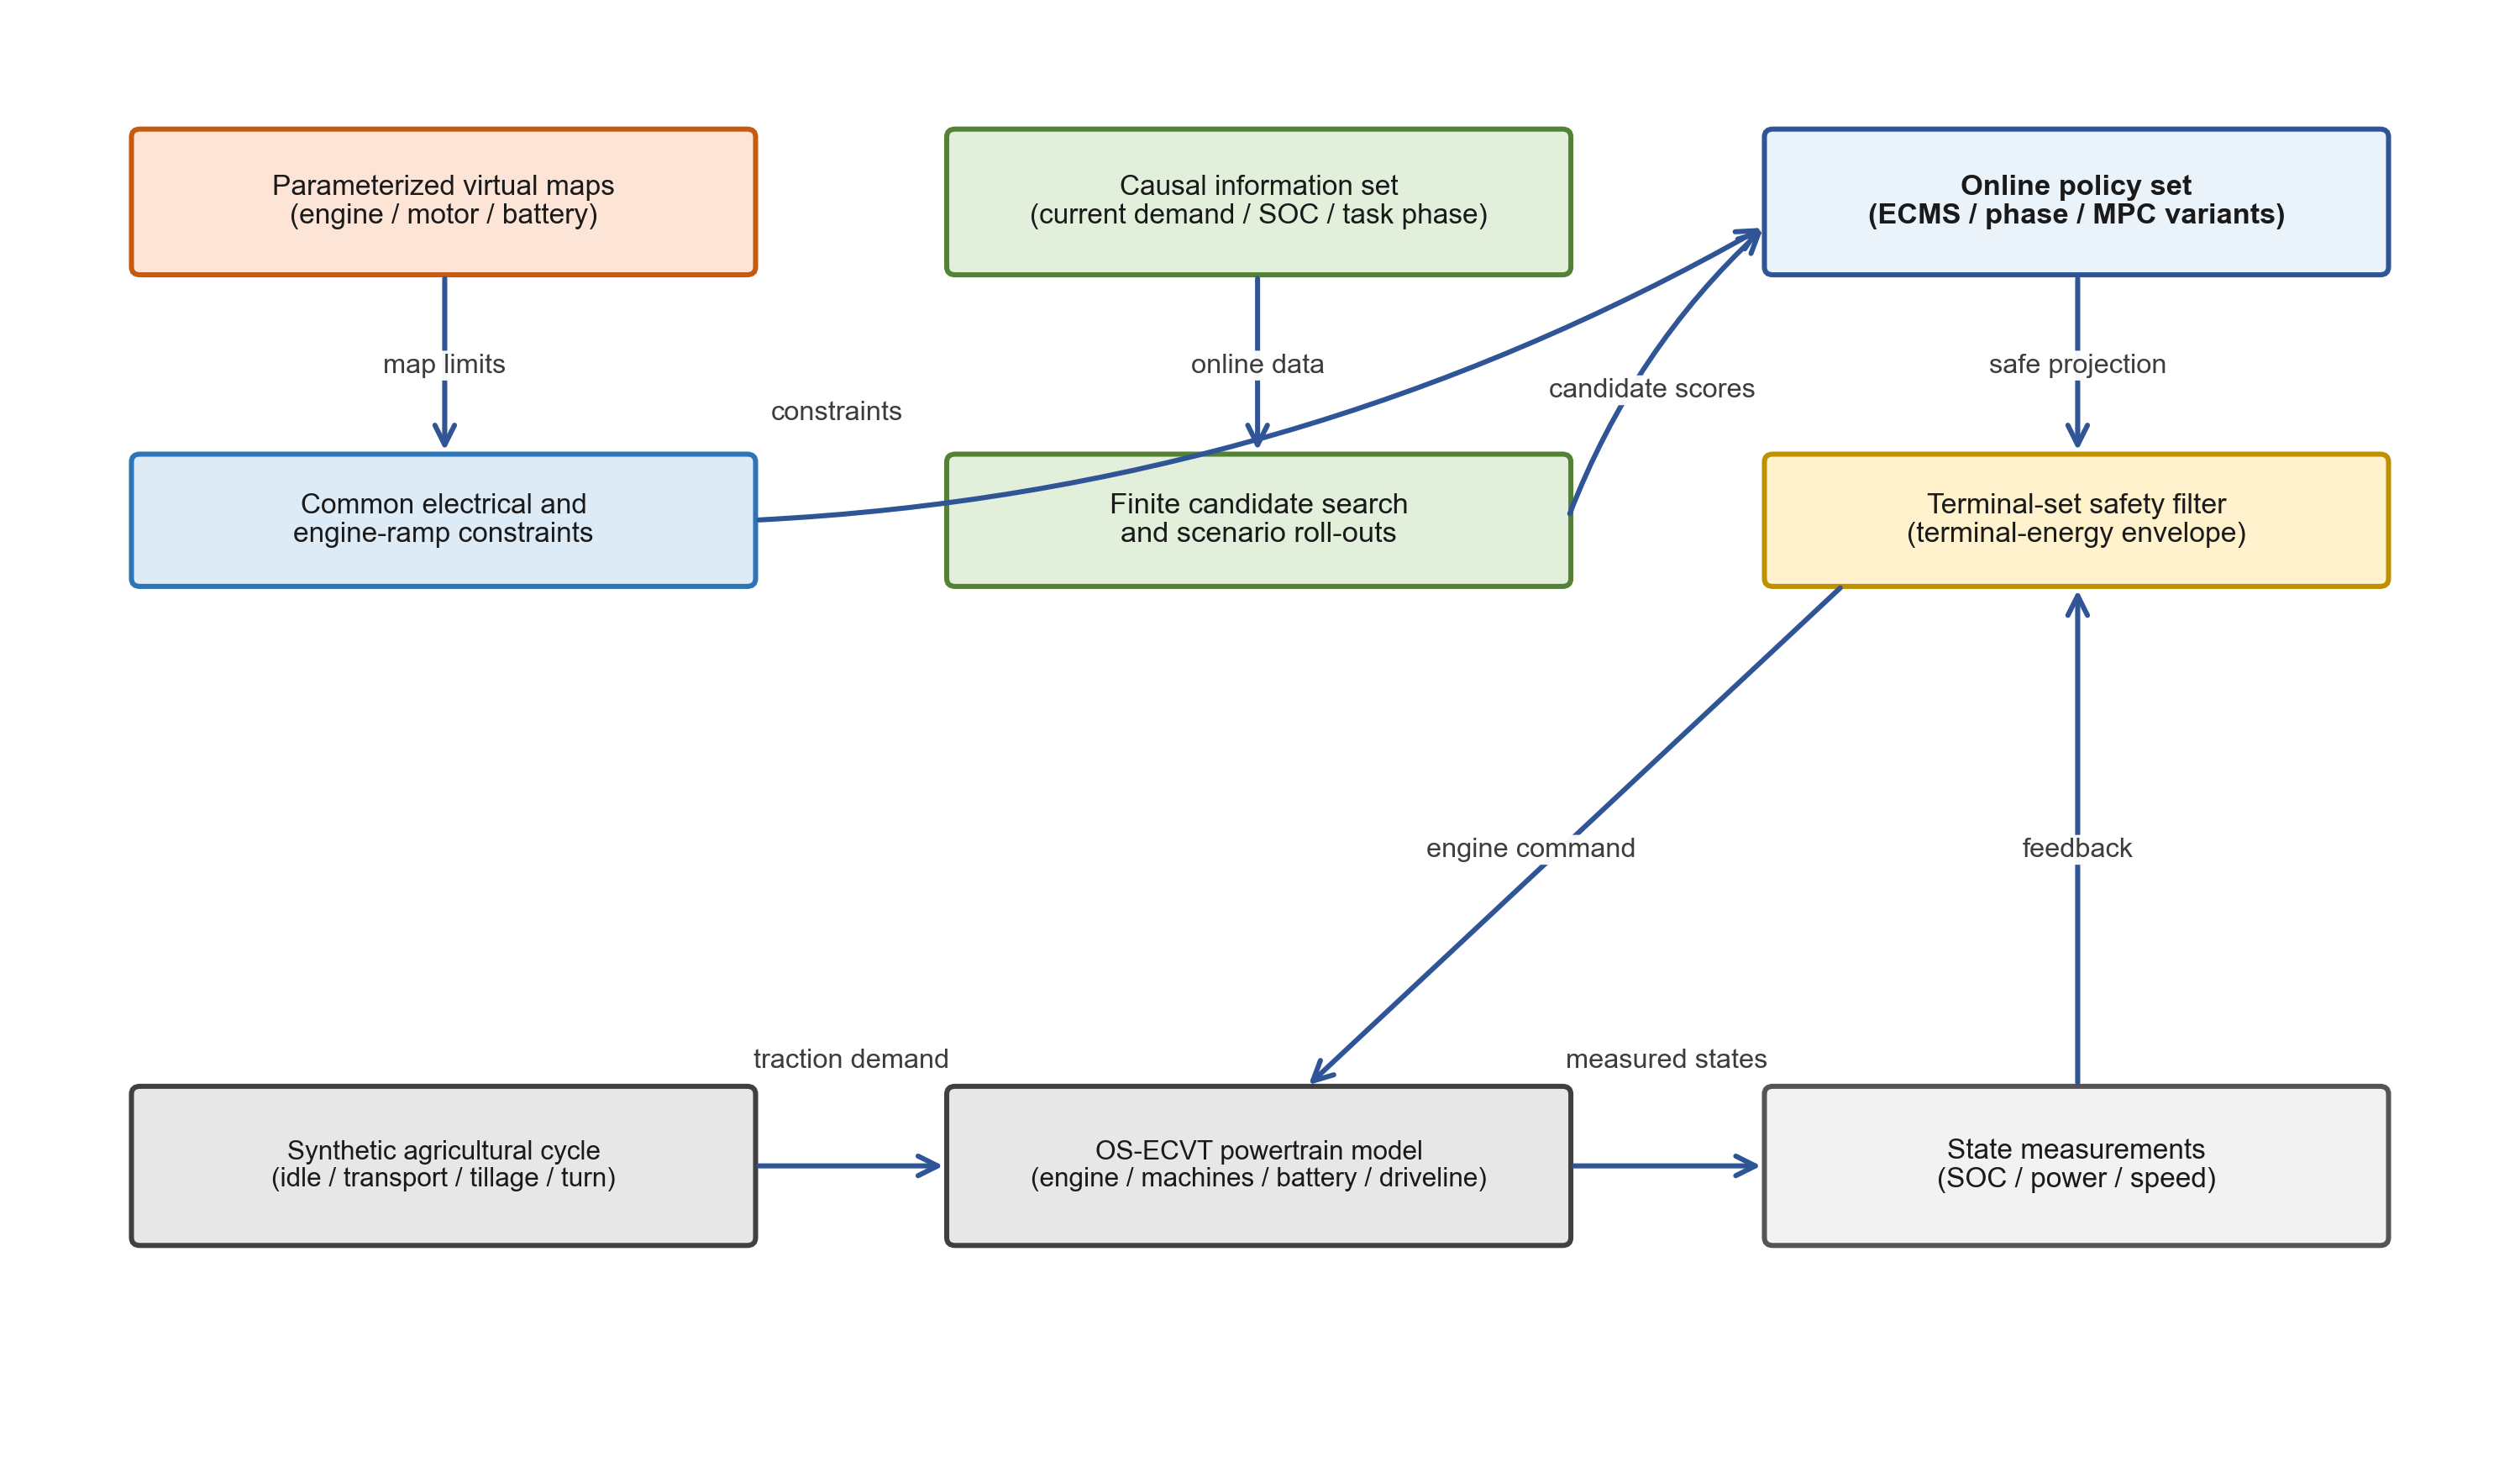
\includegraphics[width=0.96\linewidth]{paper2_architecture.png}
\caption{Strictly causal controller-comparison architecture for the virtual prototype. The online methods share the same plant, terminal-energy governor, and hard constraints.}
\label{fig:architecture}
\end{figure}

\subsection{Protocols and validity rule}
All primary simulations use a 0.1 s sample time, a 600 s stochastic agricultural cycle, and $SOC_0=0.55$. The common virtual platform has a 300 kW engine, a 200 kWh battery, 150 kW motor and battery-bus limits, a 60 kW stable engine-power floor, and a 40 kW s$^{-1}$ applied engine-power ramp. The engineering out-of-the-loop (OOL) baseline uses the same accessory demand, terminal governor, and plant constraints as every online controller. A run is strictly valid only when $|SOC_T-SOC_0|\le10^{-4}$, maximum traction shortage is no more than 1 W, and motor, battery-bus, proxy MG, speed, and applied-ramp violations are no more than 1 W or rpm. MPC results are additionally certified only when experiment-runner finite-candidate fallback and forecast ramp-envelope infeasibility are both zero. Terminal-set MPC must additionally have zero terminal-set violations; its internal safety-filter activations are reported rather than excluded. A low-fuel run outside either rule is not counted as a saving.

The primary arm uses a literature-shaped engine map derived from the published Deutz BF 6M 2012 C consumption-regression shape \cite{devyanin2023}, rescaled to a 300 kW, 42\% peak-efficiency virtual platform. It is literature-shaped rather than calibrated for a target tractor. A second arm replaces only the engine efficiency shape with a deliberately steep low-load island (efficiency 0.08 at zero load); it retains the same 300 kW platform, cycle, battery, electrical limits, and controller settings. This is a mechanism sensitivity, not a robustness or hardware-validation test.

The stochastic disturbance scale is 0.25 and its 10 s random-walk targets are continuously interpolated, consistent with the actuator-rate limit. Seeds 2200--2205 form the development set. Ten predeclared ECMS factors ($\lambda=0.5,0.75,1.0,1.25,1.5,2.0,2.5,3.0,4.0,5.0$) are eligible only if all six development runs are strictly valid, and the lowest mean-fuel eligible factor is frozen. The resulting factor is evaluated once on the disjoint 20-seed test set (2220--2239), together with the unmodified phase policy and frozen MPC settings. No test-set result is used to choose a controller setting.

\subsection{Predeclared MPC mechanism map}
The frozen framework comparison identifies one implementation point, but cannot establish whether its fuel result is specific to horizon or forecast information. A separate, predeclared mechanism map therefore uses new development seeds 2400--2405 and new holdout seeds 2420--2439. It evaluates terminal-set scenario MPC at horizons $H=4,8,12$ under two causal information conditions: a history-only predictor, and the same predictor augmented by the public zero-disturbance task phase and the present demand measurement. The phase condition contains no future realization from an evaluated seed. The scenario count, terminal weight, 300 kW platform, two maps, dynamic OOL baseline, $10^{-4}$ SOC rule, and all hard limits are unchanged.

Within each map, only settings certified on all six development paths are eligible; the eligible setting with the greatest mean direct-fuel saving is frozen and evaluated once on all 20 holdout paths. Certification additionally requires zero experiment-runner fallback, zero forecast ramp-envelope infeasibility, and zero terminal-set violations. Internal safety-filter activations and elapsed runtime are retained as outcome measures, not used to exclude a path. All six development cells are reported, so the holdout result cannot be interpreted as a post hoc choice of a favorable horizon or preview policy.

\section{Results}
\subsection{Strict controller-framework comparison}
All test-set OOL runs and all certified controller pairs met the $10^{-4}$ terminal-SOC rule. On the literature-shaped map, the phase policy was the only controller with a positive mean, but its $0.010\%$ saving is practically negligible. Frozen map-aware ECMS increased fuel use by $0.251\%$. Deterministic MPC was strictly valid on 15/20 runs and zero-fallback certified on 8/20; scenario MPC was strictly valid on 20/20 and certified on 18/20. The terminal-set scenario MPC was strictly valid and zero-external-fallback certified on all 20 paths, with zero terminal-set violations; its internal safety filter activated 614 times (30.7 per path). Its paired fuel change was $-0.704\%$. The result closes the finite-candidate feasibility gap without concealing the intervention frequency, but the additional conservatism does not improve fuel use.

The steep-island sensitivity reverses only the ECMS result: the frozen factor $\lambda=2.0$ saved $10.491\%$ on all 20 pairs. The phase policy and all MPC variants remained fuel-inferior. Terminal-set MPC again achieved 20/20 strict and zero-external-fallback certifications with zero terminal-set violations, while its filter activated 619 times (31.0 per path) and its fuel change was $-3.219\%$. Because all virtual hardware, cycle, terminal-energy rule, and test seeds are unchanged, the contrast identifies the assumed engine-efficiency shape as the source of this virtual benefit; it does not imply a field fuel saving.

\begin{table}[H]
\centering
\caption{Strictly causal 20-seed controller comparison. Direct-fuel statistics use only strict-terminal-SOC and, for MPC, zero-experiment-runner-fallback certified pairs. Terminal-set MPC additionally has zero terminal-set violations; its safety-filter activations are reported rather than treated as excluded samples. All values are paired with the same-seed engineering OOL.}
\label{tab:framework}
\scriptsize
\setlength{\tabcolsep}{3pt}
\begin{tabular}{llrrrl}
\toprule
Engine map & Controller & Strict valid & Certified pairs & Filter steps & Saving vs. OOL (\%) \\
\midrule
Literature-shaped & Map-aware ECMS & 20/20 & 20 & -- & $-0.251$ [$-0.264$, $-0.238$] \\
Literature-shaped & Nominal phase policy & 20/20 & 20 & -- & $+0.010$ [$+0.006$, $+0.015$] \\
Literature-shaped & Deterministic MPC & 15/20 & 8 & -- & $-0.658$ [$-0.700$, $-0.615$] \\
Literature-shaped & Scenario MPC & 20/20 & 18 & -- & $-0.346$ [$-0.374$, $-0.319$] \\
Literature-shaped & Terminal-set scenario MPC & 20/20 & 20 & 614 & $-0.704$ [$-0.756$, $-0.653$] \\
\midrule
Steep-island sensitivity & Map-aware ECMS & 20/20 & 20 & -- & $+10.491$ [$+10.445$, $+10.538$] \\
Steep-island sensitivity & Nominal phase policy & 20/20 & 20 & -- & $-0.077$ [$-0.133$, $-0.021$] \\
Steep-island sensitivity & Deterministic MPC & 15/20 & 8 & -- & $-2.213$ [$-2.292$, $-2.133$] \\
Steep-island sensitivity & Scenario MPC & 20/20 & 18 & -- & $-2.529$ [$-2.785$, $-2.273$] \\
Steep-island sensitivity & Terminal-set scenario MPC & 20/20 & 20 & 619 & $-3.219$ [$-3.884$, $-2.553$] \\
\bottomrule
\end{tabular}
\end{table}

\begin{figure}[H]
\centering
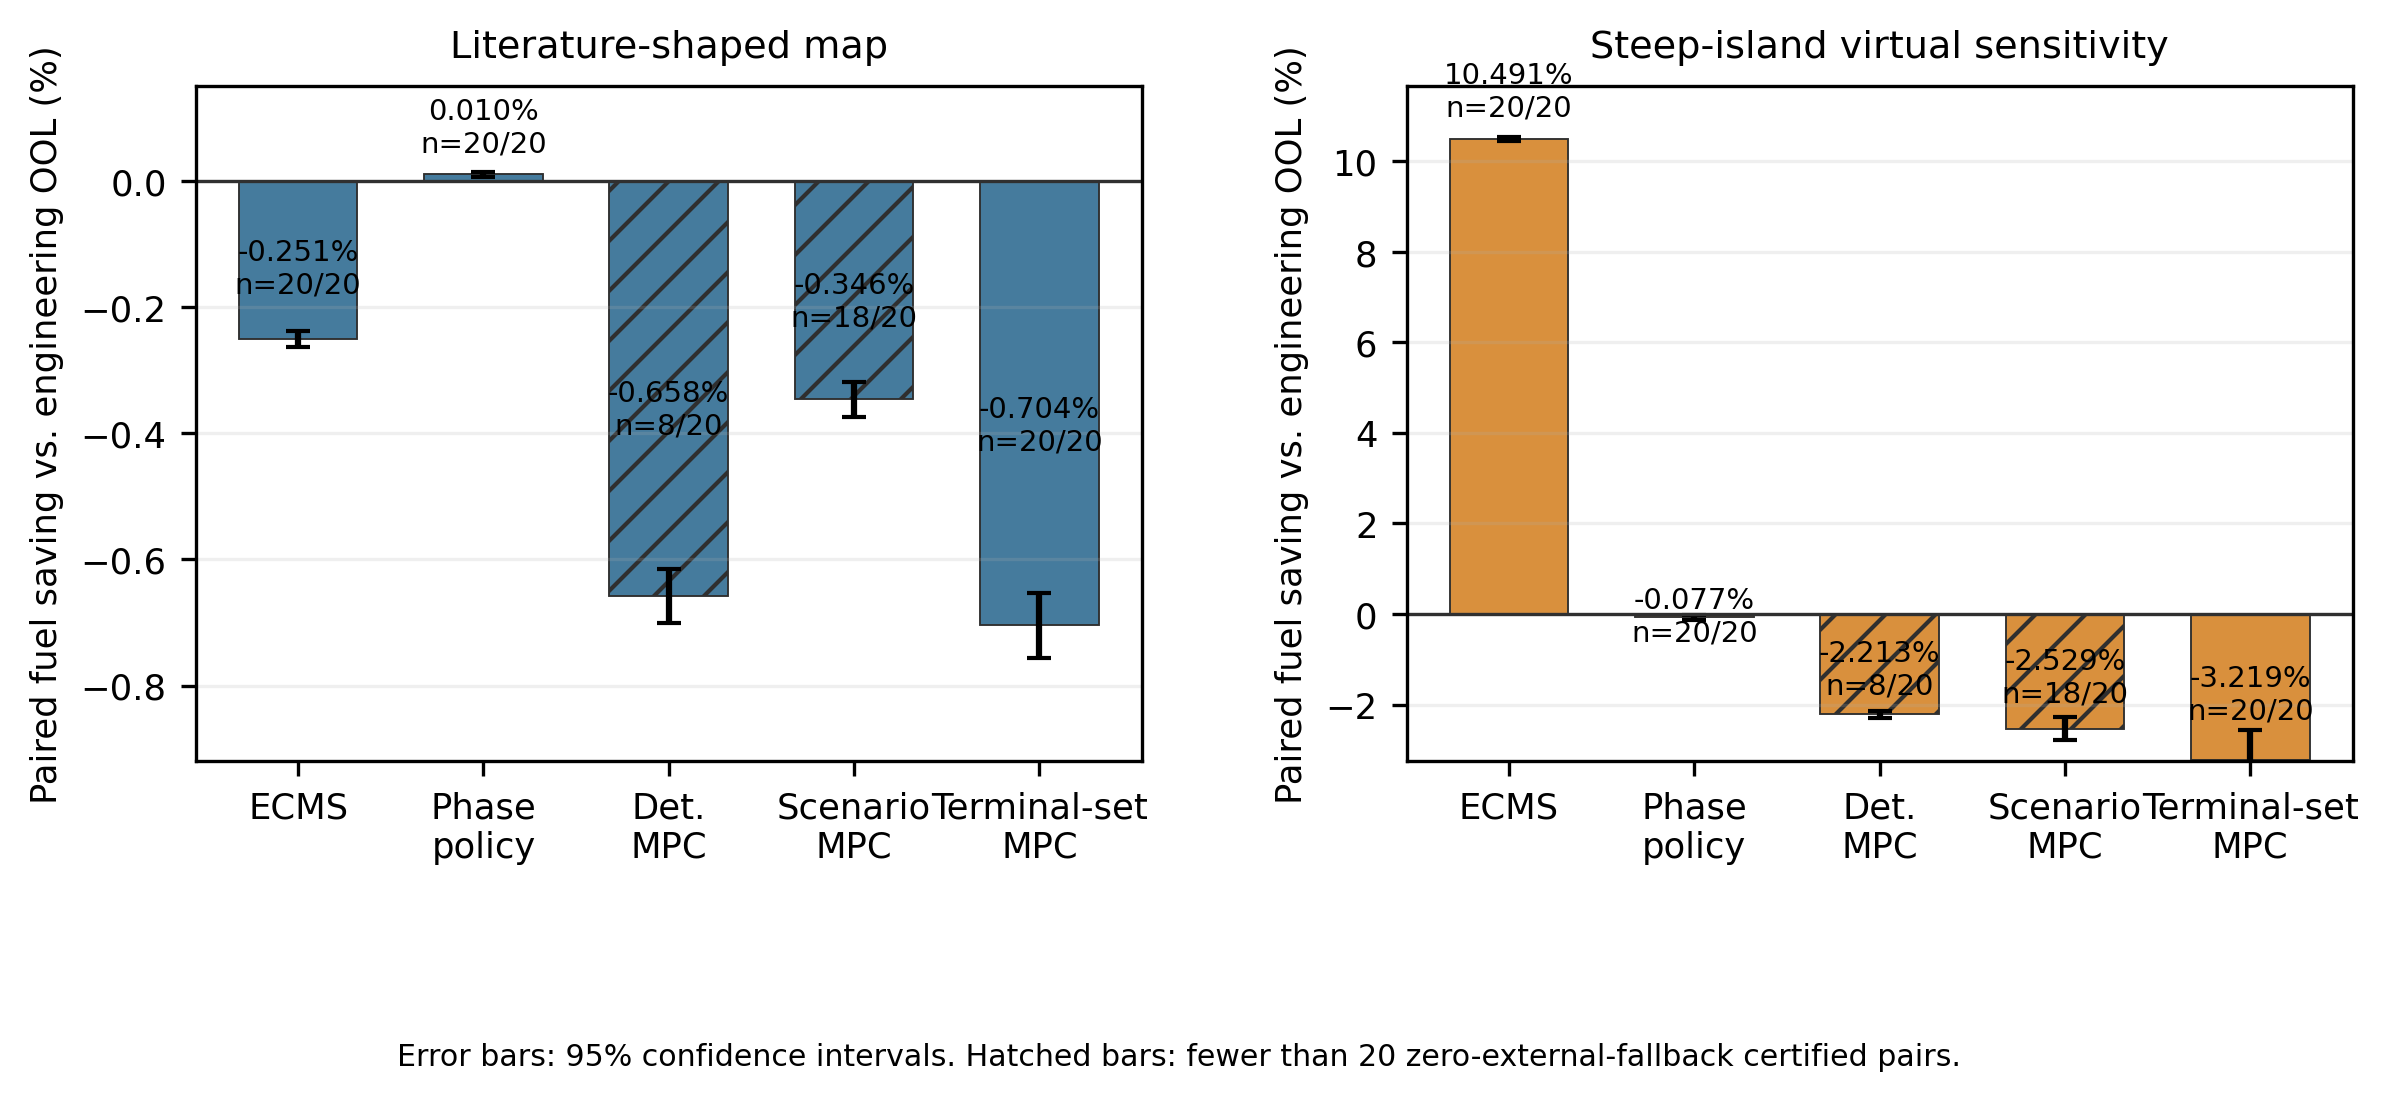
\includegraphics[width=0.98\linewidth]{paper2_controller_framework.png}
\caption{Frozen strictly causal controller comparison on the 20 unseen stochastic-cycle seeds. Error bars show 95\% confidence intervals. Hatched MPC bars have fewer than 20 zero-experiment-runner-fallback certified pairs. Terminal-set MPC has 20 certified paths in both panels; its internal filter counts appear in Table~\ref{tab:framework}. The right panel is a declared virtual-map sensitivity, not an engineering-performance estimate.}
\label{fig:framework}
\end{figure}

\subsection{Horizon--preview mechanism map}
Figure~\ref{fig:mechanism} rules out a positive terminal-set MPC result as an artifact of the original eight-sample, public-phase setting within the declared mechanism grid. On the literature-shaped map, history-only $H=8$ was the best eligible development setting ($-0.171\%$) and was frozen. Its 20/20 certified holdout result was $-0.168\%$ (95\% CI: $-0.190$ to $-0.146\%$), with no safety-filter activations and a mean runtime of 4.108 s per 600 s virtual path. The public-phase variants were more fuel-inferior and activated the filter 13.5--34.5 times per development path. History-only $H=4$ was certified on only one of six development paths.

The same selection occurred on the steep-island map: history-only $H=8$ was the closest eligible development setting to OOL ($-2.034\%$), yet its independent 20/20 holdout result was $-2.079\%$ (95\% CI: $-2.106$ to $-2.051\%$), with no filter activations and 5.059 s mean runtime. Increasing the horizon or adding the public phase did not yield a positive certified result; phase-preview $H=12$ was certified on only five of six development paths. The screen is not a claim about all MPC formulations or all cycle classes. It establishes, for the six prespecified causal settings and two declared maps, that forecast information and a longer finite horizon did not recover a fuel advantage after strict terminal-energy and feasibility accounting.

\begin{figure}[H]
\centering
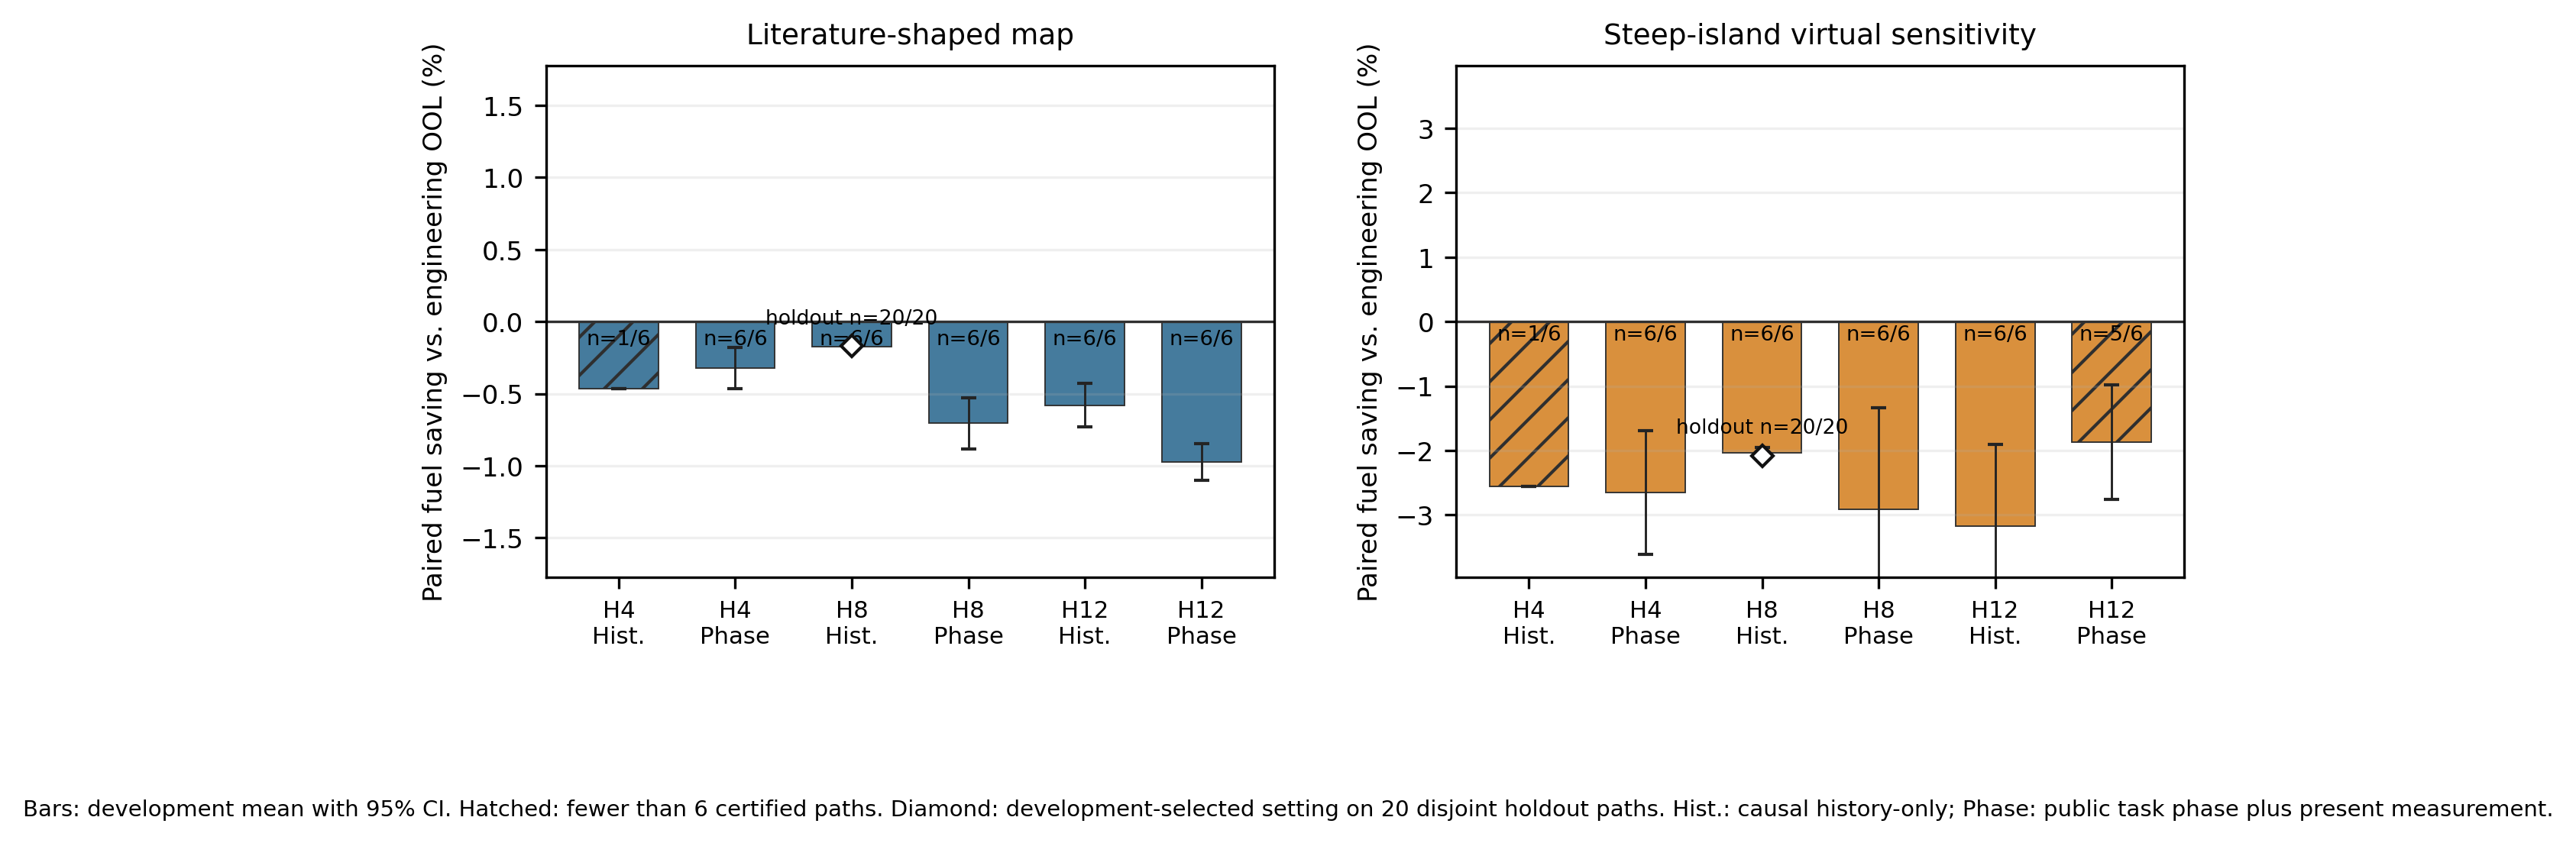
\includegraphics[width=0.98\linewidth]{paper2_mpc_mechanism_map.png}
\caption{Predeclared horizon--preview mechanism map for terminal-set scenario MPC. Bars are six-path development means with 95\% confidence intervals. Hatched bars have fewer than six certified paths. The diamond is the setting selected solely on development results and then evaluated on 20 disjoint holdout paths. ``Hist.'' uses only causal history and the present measurement; ``Phase'' adds the public nominal task phase, but no realized future sample.}
\label{fig:mechanism}
\end{figure}

\begin{table}[H]
\centering
\caption{Independent holdout check of the development-selected mechanism-map setting. The negative values are reported as fuel increases relative to the same-seed engineering OOL; they are retained to quantify the feasibility--fuel trade-off rather than suppressed.}
\label{tab:mechanism-holdout}
\scriptsize
\setlength{\tabcolsep}{3pt}
\begin{tabularx}{\linewidth}{@{}X p{0.27\linewidth} p{0.13\linewidth} p{0.30\linewidth}@{}}
\toprule
Virtual map & Development-frozen setting & Holdout (n/20) & Saving vs. OOL (\%, 95\% CI) \\
\midrule
Literature-shaped & $H=8$, history-only & 20/20 & $-0.168$ [$-0.190$, $-0.146$] \\
Steep-island sensitivity & $H=8$, history-only & 20/20 & $-2.079$ [$-2.106$, $-2.051$] \\
\bottomrule
\end{tabularx}
\end{table}

\subsection{Idealized full-information envelope}
A separate, predeclared oracle diagnostic quantifies how much favorable virtual-model headroom remains when the complete future of the smooth nominal task is known. It retains the same 300 kW platform, 200 kWh battery, 150 kW motor and battery-bus limits, 60 kW stable engine floor, 40 kW s$^{-1}$ applied ramp, wheel-side recovery, physical SOC bounds, and dynamic realistic-OOL baseline. Its only intentional idealizations are full future information and a task-level terminal SOC band of $\pm0.01$, rather than the $10^{-4}$ direct-fuel rule used above. It is therefore not included in the causal controller comparison.

Both declared map conditions were evaluated at 4 kW/0.005-SOC and 2 kW/0.002-SOC grid resolutions. The literature-shaped grid solution was rejected after continuous replay, which ended at a SOC error of $-0.0310$ and thus exceeded the declared task-level band. Under the deliberately steep low-load map, the continuous 4 kW trajectory met all hard limits and ended at a SOC error of $+0.00669$; the refined-grid raw value differed by only 0.004 percentage points. Its continuous-replay raw engine-fuel reduction was 21.611\%. However, the paired OOL ended at $+0.00950$ SOC, leaving the oracle 0.563 kWh lower. Returning that energy at a predeclared 0.42 fuel-conversion efficiency adds 0.136 L, giving an energy-normalized reduction of 19.828\%, i.e., approximately 20\% only in this idealized full-information virtual case (Table~\ref{tab:oracle}).

\begin{table}[H]
\centering
\caption{Declared full-information oracle diagnostic. These values are excluded from the strictly causal controller statistics. The raw result is shown with terminal-energy normalization so that a task-level SOC band is not mistaken for a directly comparable fuel saving.}
\label{tab:oracle}
\scriptsize
\setlength{\tabcolsep}{3pt}
\begin{tabularx}{\linewidth}{@{}X p{0.23\linewidth} p{0.14\linewidth} p{0.20\linewidth}@{}}
\toprule
Virtual map & Continuous result & Raw saving (\%) & Normalized saving (\%) \\
\midrule
Literature-shaped & Rejected: terminal SOC error $-0.0310$ & -- & -- \\
Steep low-load sensitivity & All hard limits satisfied & $+21.611$ & $+19.828$ \\
\bottomrule
\end{tabularx}
\end{table}

\subsection{Excluded full-information diagnostics}
Earlier full-future dynamic-programming and looser-terminal-SOC explorations are retained in the reproducibility archive as diagnostic audits only. They are excluded from this article's online comparison because full future demand, grid-terminal feasibility, or residual terminal battery energy can produce fuel figures that are not available to a causal controller. In particular, a former 24.087\% grid value failed continuous SOC replay and is not reported as a result. The causal controller statistics above use the common $10^{-4}$ terminal-SOC threshold exclusively.

\section{Discussion}
The literature-shaped arm does not support a meaningful fuel-saving effect from any tested causal controller. The $0.010\%$ phase-policy difference is statistically separated from zero in this deterministic virtual protocol but is too small to be engineering-significant. The terminal-set formulation demonstrates the central feasibility trade-off: it eliminates external fallback and terminal-set violations on all tested paths, but its 614 safety projections increase fuel use relative to the already fuel-inferior scenario MPC. These outcomes do not demonstrate that MPC is intrinsically unsuitable for tractor energy management; they show that recursive feasibility and fuel optimality are separate design requirements in this finite-set implementation.

The steep-island arm supplies a more informative mechanism result than a controller ranking alone. Its large ECMS effect is achieved without future demand and under the same terminal-energy and hardware rules, but it disappears when the engine map is replaced by the literature-shaped arm. The result therefore attributes the virtual saving to the assumed low-load efficiency penalty and the associated opportunity for load shifting. It must not be interpreted as an estimate for a physical tractor, and it would be inappropriate to select the 10.491\% number as a headline performance result.

The horizon--preview map separates the central negative result from a single arbitrary MPC setting. Both development procedures selected history-only $H=8$, and both independent holdout results remained negative with 20/20 certification. The failure of public-phase variants to improve fuel use is particularly informative: in this finite-set implementation, the additional phase prior caused more safety projections without an offsetting map-aware load-shifting gain. This does not prove that preview is universally detrimental. It bounds the conclusion to the declared horizons, predictor, cycle, virtual maps, and terminal-set construction, while ruling out an unsupported claim that modest causal preview or a longer tested horizon restores MPC fuel savings.

The full-information oracle makes the same distinction from another direction. The approximately 20\% energy-normalized value requires both the declared steep low-load map and future knowledge of the entire smooth nominal task; the literature-shaped counterpart did not survive continuous terminal-SOC replay. It measures virtual headroom, not a causal-controller target. Reporting both raw and normalized values is necessary because the task-level terminal band otherwise permits unequal residual battery energy.

This is a theoretical simulation, so target-platform calibration and field measurements are not prerequisites for the internal validity of its declared virtual model. The 300 kW component maps, battery model, planetary relation, MG constraints, and stochastic cycle are defined model inputs and must be preserved with the source code and parameter tables. The literature-shaped map uses the load trend of a 155 kW Deutz engine only as a transparent reference shape before rescaling; the steep island is a deliberately specified mechanism map. Their absence of target-platform calibration limits only external generalization, not the stated conditional virtual-model findings. The remaining methodological priorities are component-map parameter ranges and sensitivity coverage, explicit admissible-demand bounds for the conditional terminal-set guarantee, and a public versioned code/data archive. Any future engineering-performance study would additionally require matched measured maps, drivetrain limits, and field cycles.

\section{Conclusions}
This study established a strict causal comparison of map-aware ECMS, a public-phase policy, deterministic MPC, scenario MPC, and terminal-set scenario MPC in a hybrid-tractor virtual prototype. The common protocol requires a $10^{-4}$ terminal-SOC error, the same applied engine dynamics, common electrical and proxy-machine limits, and same-seed OOL pairing. The terminal-set formulation achieved 20/20 zero-external-fallback and zero-terminal-set-violation paths on both declared maps, but increased fuel use by 0.704\% on the literature-shaped map and 3.219\% on the steep-island map. A predeclared horizon--preview map selected history-only $H=8$ on new development seeds; its 20/20 holdout fuel changes remained $-0.168\%$ and $-2.079\%$. Under the same maps, frozen ECMS changed fuel use by $-0.251\%$ and $+10.491\%$, respectively. A separate full-information, $\pm0.01$-SOC oracle reached 21.611\% raw and 19.828\% terminal-energy-normalized reduction only on the declared steep low-load virtual map; it is an approximately 20\% headroom diagnostic, not an online result. Therefore, the evidence supports a conditional recursive-feasibility construction, map-sensitivity audit, a measured horizon--preview boundary, and an explicitly bounded idealized envelope, not a generic MPC advantage or a hardware-performance estimate. The defined virtual component maps are sufficient for this theoretical study; matched measurements are needed only before extending its conclusions to a physical platform.

\authorcontributions{Conceptualization, C.C.; Methodology, C.C.; Software, C.C.; Formal analysis, C.C.; Visualization, C.C.; Writing---original draft preparation, C.C.; Resources, C.C.; Validation, Z.Z.; Investigation, L.W.; Writing---review and editing, Z.L. and Y.Z.; Supervision, Z.L. and Y.Z.; Project administration, Y.Z.; Funding acquisition, Y.Z.}
\funding{This work has received funding from the Science and Technology Project of the Ministry of Agriculture and Rural Affairs of China.}
\institutionalreview{Not applicable.}
\informedconsent{Not applicable.}
\dataavailability{The virtual-prototype source code, reproduction scripts, including the declared full-information oracle diagnostic, and JSON outputs supporting these results are publicly available at \url{https://github.com/Fat-pig-Cui/agricultural-tractor-virtual-prototypes}. The Zenodo version DOI for the archival release will be added before publication.}
\acknowledgments{During preparation of this manuscript, the authors used OpenAI Codex for English translation, language editing, and development of plotting scripts. The authors must review and edit all output and take full responsibility for the content before submission.}
\conflictsofinterest{The authors declare no conflicts of interest.}

\begin{thebibliography}{10}
\bibitem{curiel2023} Curiel-Olivares, G.; Johnson, S.; Escobar, G.; Schacht-Rodr\'iguez, R. Model predictive control-based energy management system for a hybrid electric agricultural tractor. \emph{IEEE Access} \textbf{2023}, \emph{11}, 118801--118811. \url{https://doi.org/10.1109/ACCESS.2023.3322462}.
\bibitem{musardo2005} Musardo, C.; Rizzoni, G.; Staccia, B. A-ECMS: An adaptive algorithm for hybrid electric vehicle energy management. \emph{Proceedings of the 44th IEEE Conference on Decision and Control} 2005, 1816--1823. \url{https://doi.org/10.1109/CDC.2005.1582424}.
\bibitem{xie2016} Xie, S.; Sun, F.; He, H.; Peng, J. Plug-in hybrid electric bus energy management based on dynamic programming. \emph{Energy Procedia} \textbf{2016}, \emph{104}, 378--383. \url{https://doi.org/10.1016/j.egypro.2016.12.064}.
\bibitem{ripaccioli2010} Ripaccioli, G.; Bernardini, D.; Di Cairano, S.; Bemporad, A.; Kolmanovsky, I. A stochastic model predictive control approach for series hybrid electric vehicle power management. \emph{American Control Conference} 2010, 5844--5849. \url{https://doi.org/10.1109/ACC.2010.5530504}.
\bibitem{mocera2020} Mocera, F.; Som\`a, A. Analysis of a parallel hybrid electric tractor for agricultural applications. \emph{Energies} \textbf{2020}, \emph{13}, 3055. \url{https://doi.org/10.3390/en13123055}.
\bibitem{mocera2020b} Mocera, F. A model-based design approach for a parallel hybrid electric tractor energy management strategy using hardware in the loop technique. \emph{Vehicles} \textbf{2020}, \emph{3}, 1--19. \url{https://doi.org/10.3390/vehicles3010001}.
\bibitem{jilek2008} J\'ilek, L.; Pra\v{z}an, R.; Podp\v{e}ra, V.; Gerndtov\'a, I. The effect of the tractor engine rated power on diesel fuel consumption during material transport. \emph{Research in Agricultural Engineering} \textbf{2008}, \emph{54}, 1--8. \url{https://doi.org/10.17221/710-RAE}.
\bibitem{janulevicius2010} Janulevi\v{c}ius, A.; Juostas, A.; Pupinis, G. Tractor engine load and fuel consumption in road construction works. \emph{Transport} \textbf{2010}, \emph{25}, 403--410. \url{https://doi.org/10.3846/transport.2010.50}.
\bibitem{huo2018} Huo, Y.; Yan, F. A predictive energy management strategy for hybrid electric powertrain with a turbocharged diesel engine. \emph{Journal of Dynamic Systems, Measurement, and Control} \textbf{2018}, \emph{140}, 061017. \url{https://doi.org/10.1115/1.4039216}.
\bibitem{devyanin2023} Devyanin, S.N.; Bizhaev, A.V.; Pavlov, Y.D.; Vetrova, S.M.; Barchukova, A.S. Parametric characterization of a tractor engine by specific fuel consumption. \emph{Agricultural Machinery and Technologies} \textbf{2023}, \emph{17}, 68--74. \url{https://doi.org/10.22314/2073-7599-2023-17-4-68-74}.
\end{thebibliography}
\end{document}
